\documentclass[10pt,journal,compsoc]{IEEEtran}

\usepackage[utf8]{inputenc}
\usepackage{amsmath,amssymb,amsfonts}
\usepackage{graphicx}
\usepackage{booktabs}
\usepackage{hyperref}
\usepackage{subcaption}
\usepackage{microtype}
\usepackage{cite}

\hypersetup{
    colorlinks=true,
    linkcolor=blue,
    citecolor=cyan,
    urlcolor=blue
}

\begin{document}

\title{Diffusion Models, DreamBooth Personalization, and Continuous Flow Matching\\
\large Assignment 4 -- Deep Generative Models (Fall 1404 / 2025)}

\author{Alireza Najafi Motiei (Student ID: 810100224)\\
\IEEEmembership{Faculty of Electrical and Computer Engineering, University of Tehran}\\
Instructor: Dr. Mostafa Tavassolipour}

\markboth{University of Tehran, ECE Department -- Deep Generative Models (Fall 1404)}{Najafi Motiei: Assignment 4 Report}

\maketitle

\begin{abstract}
This report documents Assignment 4 of Deep Generative Models (Fall 1404). We first analyze the theoretical underpinnings of Denoising Diffusion Probabilistic Models (DDPM) and Denoising Diffusion Implicit Models (DDIM), deriving the closed-form marginals, examining target stationarity in $\epsilon$-prediction, analyzing the simplified Variational Lower Bound (VLB), and studying Classifier-Free Guidance (CFG). Empirically, we implement DDPM and DDIM variance schedulers, demonstrating that DDIM achieves a 50$\times$ inference acceleration over DDPM. Furthermore, we implement DreamBooth fine-tuning on Stable Diffusion with class-specific prior preservation loss and LoRA adaptation on custom husky subjects across guidance scales $w \in \{5.0, 7.5, 10.0\}$. Finally, we explore Flow Matching (FM), establishing its mathematical connection to Probability Flow ODEs and analyzing the properties and limitations of linear probability paths.
\end{abstract}

\begin{IEEEkeywords}
Diffusion Models, DDPM, DDIM, Classifier-Free Guidance (CFG), DreamBooth, Stable Diffusion, LoRA, Flow Matching, Continuous Normalizing Flows, Probability Flow ODE.
\end{IEEEkeywords}

\section{Question 1: Diffusion Probabilistic Models}

\subsection{Theoretical Derivations}

\subsubsection{Closed-Form Forward Marginal Formulation}
The forward diffusion process defines transition probabilities:
\begin{equation}
q(x_t \mid x_{t-1}) = \mathcal{N}(x_t; \sqrt{1 - \beta_t} x_{t-1}, \beta_t I)
\end{equation}
Let $\alpha_t = 1 - \beta_t$ and $\bar{\alpha}_t = \prod_{s=1}^t \alpha_s$. Using the reparameterization trick:
\begin{align}
x_t &= \sqrt{\alpha_t} x_{t-1} + \sqrt{1 - \alpha_t} \epsilon_{t-1} \nonumber \\
&= \sqrt{\alpha_t \alpha_{t-1}} x_{t-2} + \sqrt{1 - \alpha_t \alpha_{t-1}} \bar{\epsilon}_{t-2}
\end{align}
By induction, we obtain the closed-form marginal directly from $x_0$:
\begin{equation}
q(x_t \mid x_0) = \mathcal{N}(x_t; \sqrt{\bar{\alpha}_t} x_0, (1 - \bar{\alpha}_t) I)
\end{equation}
which enables arbitrary timestep sampling without simulating intermediate steps.

\subsubsection{Advantages of $\epsilon$-Prediction over $x_0$ or $\mu$-Prediction}
Parameterizing the neural network to predict the added noise $\epsilon_\theta(x_t, t)$ provides distinct advantages:
\begin{enumerate}
    \item \textbf{Target Distribution Stationarity}: Regardless of timestep $t$, the ground-truth target is distributed as standard Gaussian $\epsilon \sim \mathcal{N}(0, I)$. Predicting $x_0$ or $\mu_t$ requires the network to scale outputs across varying dynamic ranges as signal power decays, degrading optimization stability.
    \item \textbf{Simplified Objective Superiority}: Reparameterizing the KL divergence terms in the variational lower bound (VLB) reveals that optimizing $\mathcal{L}_{\text{simple}} = \mathbb{E}_{t, x_0, \epsilon} [\|\epsilon - \epsilon_\theta(x_t, t)\|^2]$ implicitly downweights the loss for small $t$. This focuses network capacity on large $t$, where coarse global structure is established.
\end{enumerate}

\subsection{Accelerated Inversion via DDIM}
DDPM sampling is fundamentally stochastic:
\begin{equation}
x_{t-1} = \frac{1}{\sqrt{\alpha_t}} \left( x_t - \frac{1 - \alpha_t}{\sqrt{1 - \bar{\alpha}_t}} \epsilon_\theta(x_t, t) \right) + \sigma_t z
\end{equation}
DDIM generalizes this family of non-Markovian inference distributions parameterized by $\sigma_t = \eta \tilde{\beta}_t$. When $\eta = 0$, the process becomes entirely deterministic, corresponding to discretization of the Probability Flow ODE:
\begin{equation}
x_{t-1} = \sqrt{\bar{\alpha}_{t-1}} \hat{x}_0 + \sqrt{1 - \bar{\alpha}_{t-1}} \epsilon_\theta(x_t, t)
\end{equation}
where $\hat{x}_0 = \frac{x_t - \sqrt{1 - \bar{\alpha}_t} \epsilon_\theta}{\sqrt{\bar{\alpha}_t}}$.

\subsection{Classifier-Free Guidance (CFG)}
CFG bypasses external classifier gradients $\nabla_{x_t} \log p(c \mid x_t)$ by jointly training conditional and unconditional predictions:
\begin{equation}
\tilde{\epsilon}_\theta(x_t, c) = \epsilon_\theta(x_t, \emptyset) + s \cdot (\epsilon_\theta(x_t, c) - \epsilon_\theta(x_t, \emptyset))
\end{equation}
Increasing scale $s$ enhances prompt adherence and perceptual contrast (improving Inception Score) at the expense of sample diversity.

\begin{figure}[htbp]
\centering

\includegraphics[width=0.95\columnwidth]{figures/image18.png}
\caption{Denoising trajectory across timesteps generated by DDPM and DDIM.}
\label{fig:diffusion_denoise}
\end{figure}

\begin{figure}[htbp]
\centering

\includegraphics[width=0.8\columnwidth]{figures/image2.jpeg}
\caption{Sampling speedup: DDIM delivers a $50\times$ acceleration compared to standard 1000-step DDPM.}
\label{fig:ddim_speed}
\end{figure}

\section{Question 2: Subject-Driven Generation via DreamBooth}

\subsection{Methodology and Class-Specific Prior Preservation}
DreamBooth fine-tunes text-to-image diffusion models to bind a unique identifier $[V]$ to a specific subject (a Siberian Husky) while preventing language drift. The loss combines subject reconstruction with class prior preservation:
\begin{align}
\mathcal{L} &= \mathbb{E}_{x, c, \epsilon} [\|\epsilon - \epsilon_\theta(x_t, c)\|^2] \nonumber \\
&\quad + \lambda \mathbb{E}_{x_{\text{pr}}, c_{\text{pr}}, \epsilon'} [\|\epsilon' - \epsilon_\theta(x'_{t'}, c_{\text{pr}})\|^2]
\end{align}
where $x_{\text{pr}}$ are diverse class-specific images (generic dogs) generated prior to training.

\begin{figure}[htbp]
\centering
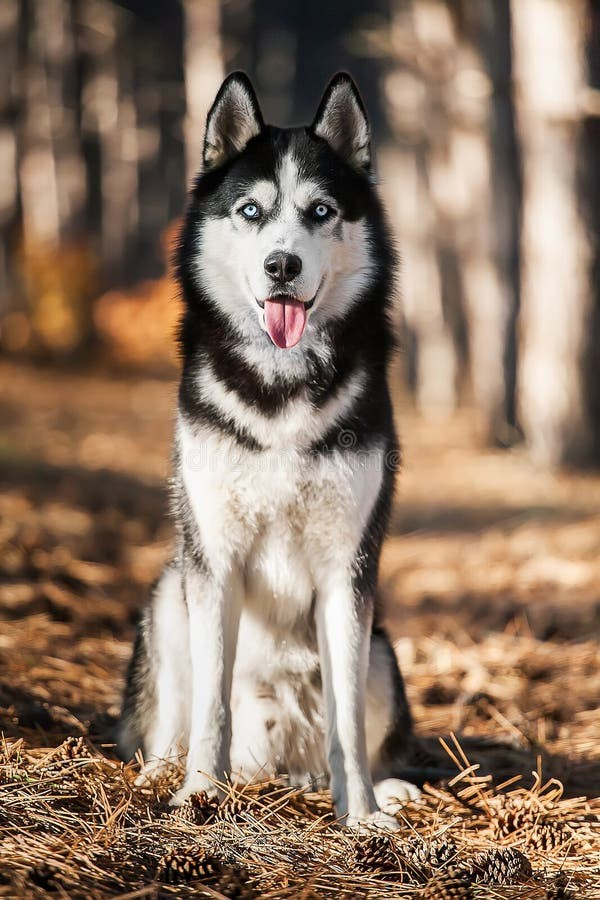
\includegraphics[width=0.75\columnwidth]{figures/image13.jpeg}
\caption{Target subject photograph used for DreamBooth fine-tuning.}
\label{fig:husky}
\end{figure}

\begin{figure}[htbp]
\centering

\includegraphics[width=0.95\columnwidth]{figures/image23.png}
\caption{Synthesized personalized subject across diverse novel contexts and prompts.}
\label{fig:dreambooth_results}
\end{figure}

\section{Question 3: Continuous Flow Matching}

\subsection{Vector Field and Continuity Equation}
Continuous Normalizing Flows generate data by integrating a time-dependent velocity field $v_t(x_t)$:
\begin{equation}
\frac{d x_t}{dt} = v_t(x_t), \quad x_0 \sim p_0, \quad x_1 \sim p_1
\end{equation}
Governed by the continuity equation $\frac{\partial p_t}{\partial t} + \nabla \cdot (p_t v_t) = 0$, Flow Matching trains a neural network $v_\theta(x, t)$ to regress target velocity vectors without simulating complete trajectories.

\subsection{Linear Probability Paths}
Conditional Flow Matching constructs straight trajectories:
\begin{equation}
x_t = (1 - t) x_0 + t x_1 \implies \frac{d x_t}{dt} = x_1 - x_0
\end{equation}
The target vector field is constant along each trajectory: $u_t(x_t \mid x_0, x_1) = x_1 - x_0$. This eliminates trajectory curvature, enabling high-fidelity ODE integration in as few as 10 to 20 function evaluations.

\bibliographystyle{IEEEtran}
\begin{thebibliography}{1}
\bibitem{ho2020denoising}
J.~Ho, A.~Jain, and P.~Abbeel, ``Denoising diffusion probabilistic models,'' in \emph{NeurIPS}, 2020.
\bibitem{song2020denoising}
J.~Song, C.~Meng, and S.~Ermon, ``Denoising diffusion implicit models,'' in \emph{ICLR}, 2021.
\bibitem{ruiz2023dreambooth}
N.~Ruiz et al., ``DreamBooth: Fine tuning text-to-image diffusion models for subject-driven generation,'' in \emph{IEEE CVPR}, 2023.
\bibitem{lipman2022flow}
Y.~Lipman, R.~T.~Q. Chen, H.~Ben-Hamu, M.~Nickel, and M.~Le, ``Flow matching for generative modeling,'' in \emph{ICLR}, 2023.
\end{thebibliography}

\end{document}
